\documentclass[tikz,border=10pt]{standalone}
\usepackage{tikz}
\usetikzlibrary{calc}

\begin{document}
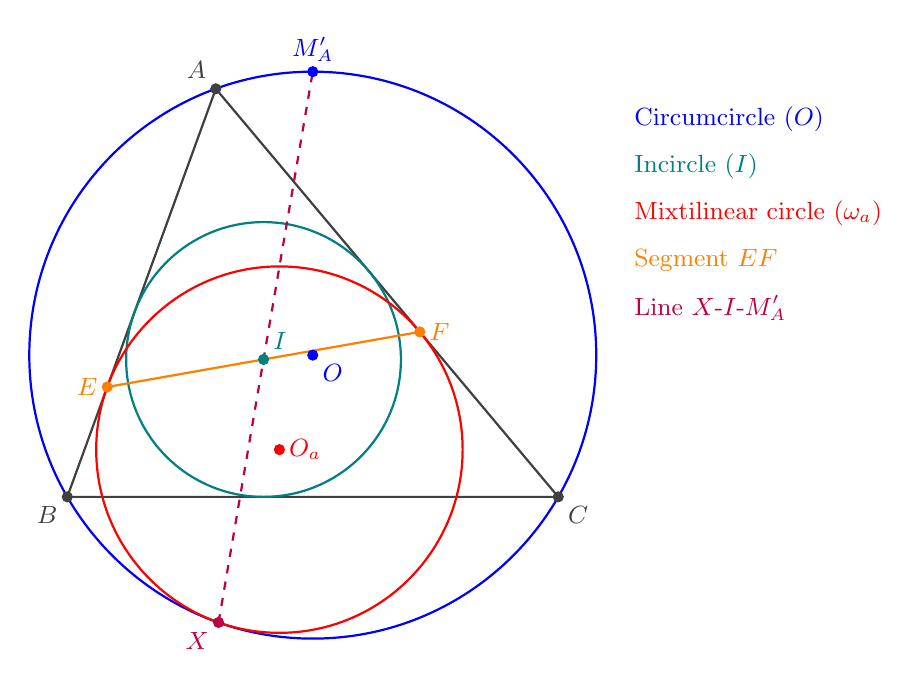
\begin{tikzpicture}[scale=1.2, font=\small]

% Circumcircle (blue)
\draw[blue, thick] (0,0) circle (3);

% Triangle ABC (dark gray)
\draw[darkgray, thick] (-1.026, 2.819) -- (-2.598, -1.5) -- (2.598, -1.5) -- cycle;

% Incircle (teal)
\draw[teal, thick] (-0.521, -0.046) circle (1.454);

% A-mixtilinear circle (red)
\draw[red, thick] (-0.353, -1.0) circle (1.939);

% Segment EF (orange)
\draw[orange, thick] (-2.175, -0.337) -- (1.133, 0.246);

% Line from X through I to M'_A (dashed purple)
\draw[purple, dashed, thick] (-0.997, -2.829) -- (-0.521, -0.046) -- (0, 3);

% Plot and label points
% O - center of circumcircle
\filldraw[blue] (0,0) circle (1.5pt);
\node[blue, below right] at (0,0) {$O$};

% A
\filldraw[darkgray] (-1.026, 2.819) circle (1.5pt);
\node[darkgray, above left] at (-1.026, 2.819) {$A$};

% B
\filldraw[darkgray] (-2.598, -1.5) circle (1.5pt);
\node[darkgray, below left] at (-2.598, -1.5) {$B$};

% C
\filldraw[darkgray] (2.598, -1.5) circle (1.5pt);
\node[darkgray, below right] at (2.598, -1.5) {$C$};

% I - incenter
\filldraw[teal] (-0.521, -0.046) circle (1.5pt);
\node[teal, above right] at (-0.521, -0.046) {$I$};

% E - tangent point on AB
\filldraw[orange] (-2.175, -0.337) circle (1.5pt);
\node[orange, left] at (-2.175, -0.337) {$E$};

% F - tangent point on AC
\filldraw[orange] (1.133, 0.246) circle (1.5pt);
\node[orange, right] at (1.133, 0.246) {$F$};

% X - tangent point on circumcircle
\filldraw[purple] (-0.997, -2.829) circle (1.5pt);
\node[purple, below left] at (-0.997, -2.829) {$X$};

% M'_A - midpoint of arc BC containing A
\filldraw[blue] (0, 3) circle (1.5pt);
\node[blue, above] at (0, 3) {$M'_A$};

% O_a - center of mixtilinear circle
\filldraw[red] (-0.353, -1.0) circle (1.5pt);
\node[red, right] at (-0.353, -1.0) {$O_a$};

% Legend
\node[blue, anchor=west] at (3.3, 2.5) {Circumcircle $(O)$};
\node[teal, anchor=west] at (3.3, 2.0) {Incircle $(I)$};
\node[red, anchor=west] at (3.3, 1.5) {Mixtilinear circle $(\omega_a)$};
\node[orange, anchor=west] at (3.3, 1.0) {Segment $EF$};
\node[purple, anchor=west] at (3.3, 0.5) {Line $X$-$I$-$M'_A$};

\end{tikzpicture}
\end{document}